%package list
\documentclass{article}
\usepackage[top=3cm, bottom=3cm, outer=3cm, inner=3cm]{geometry}
\usepackage{graphicx}
\usepackage{url}
%\usepackage{cite}
\usepackage{hyperref}
\usepackage{array}
%\usepackage{multicol}
\newcolumntype{x}[1]{>{\centering\arraybackslash\hspace{0pt}}p{#1}}
\usepackage{natbib}
\usepackage{pdfpages}
\usepackage{multirow}
\usepackage{multirow}
\usepackage[normalem]{ulem}
\useunder{\uline}{\ul}{}
\usepackage{amsmath}
\usepackage{float}
\usepackage{multicol}
\usepackage{subcaption}


% para tener url cortas en bib
\let\oldUrl\url
\renewcommand{\url}[1]{\href{#1}{Enlace}}
%

%%%%%%%%%%%%%%%%%%%%%%%%%%%%%%%%%%%%%%%%%%%%%%%%%%%%%%%%%%%%%%%%%%%%%%%%%%%%
%%%%%%%%%%%%%%%%%%%%%%%%%%%%%%%%%%%%%%%%%%%%%%%%%%%%%%%%%%%%%%%%%%%%%%%%%%%%
\newcommand{\csemail}{vmachacaa@ulasalle.edu.pe}
%\newcommand{\csdocente}{MSc. Vicente Enrique Machaca Arceda}
\newcommand{\csdocente}{
    Vicente Machaca Arceda \\
    Enzo Velásquez Lobatón \\
	Carlo Corrales Delgado\\
	Oscar Ramirez Valdez
	}
\newcommand{\cscurso}{Computación de Alto Desempeño}
\newcommand{\csuniversidad}{Universidad Nacional de San Agustín de Arequipa}
\newcommand{\csescuela}{Doctorado en Ciencias de la Computación}
\newcommand{\cspracnr}{03}
\newcommand{\cstema}{Plataforma distribuída con Spark para el análisis de secuencias Next-generation}
%%%%%%%%%%%%%%%%%%%%%%%%%%%%%%%%%%%%%%%%%%%%%%%%%%%%%%%%%%%%%%%%%%%%%%%%%%%%
%%%%%%%%%%%%%%%%%%%%%%%%%%%%%%%%%%%%%%%%%%%%%%%%%%%%%%%%%%%%%%%%%%%%%%%%%%%%


\usepackage[english,spanish]{babel}
\usepackage[utf8]{inputenc}
\AtBeginDocument{\selectlanguage{spanish}}
\renewcommand{\figurename}{Figura}
\renewcommand{\refname}{Referencias}
\renewcommand{\tablename}{Tabla} %esto no funciona cuando se usa babel
\AtBeginDocument{%
	\renewcommand\tablename{Tabla}
}

\usepackage{fancyhdr}
\pagestyle{fancy}
\fancyhf{}
\setlength{\headheight}{30pt}
\renewcommand{\headrulewidth}{1pt}
\renewcommand{\footrulewidth}{1pt}
\fancyhead[L]{\raisebox{-0.2\height}{
\includegraphics[width=3cm]{img/logo_unsa}}}
\fancyhead[C]{}
\fancyhead[R]{\fontsize{7}{7}\selectfont	\csuniversidad \\ \csescuela \\ \textbf{\cscurso} }
\fancyfoot[L]{Vicente, Enzo, Oscar y Carlos}
\fancyfoot[C]{\cscurso}
\fancyfoot[R]{Página \thepage}


% para el codigo fuente
\usepackage{listings}
\usepackage{color}
\definecolor{dkgreen}{rgb}{0,0.6,0}
\definecolor{gray}{rgb}{0.5,0.5,0.5}
\definecolor{mauve}{rgb}{0.58,0,0.82}
\lstset{frame=tb,
	language=Python,
	aboveskip=3mm,
	belowskip=3mm,
	showstringspaces=false,
	columns=flexible,
	basicstyle={\small\ttfamily},
	numbers=none,
	numberstyle=\tiny\color{gray},
	keywordstyle=\color{blue},
	commentstyle=\color{dkgreen},
	stringstyle=\color{mauve},
	breaklines=true,
	breakatwhitespace=true,
	tabsize=3
}




\begin{document}
	
	
	
	
\begin{titlepage}
	
	\newcommand{\HRule}{\rule{\linewidth}{0.5mm}} % Defines a new command for the horizontal lines, change thickness here
	
	\center % Center everything on the page
	
	%----------------------------------------------------------------------------------------
	%	HEADING SECTIONS
	%----------------------------------------------------------------------------------------
	
	\textsc{\LARGE \csuniversidad}\\[1.5cm] % Name of your university/college
	\textsc{\Large \cscurso}\\[0.5cm] % Major heading such as course name
	%\textsc{\large Assignment 1}\\[0.5cm] % Minor heading such as course title
	
	%----------------------------------------------------------------------------------------
	%	TITLE SECTION
	%----------------------------------------------------------------------------------------
	
	\vspace{2cm}
	
	\HRule \\[0.4cm]
	{ \huge \bfseries \cstema}\\[0.4cm] % Title of your document
	\HRule \\[1.5cm]
	
	%----------------------------------------------------------------------------------------
	%	AUTHOR SECTION
	%----------------------------------------------------------------------------------------
	
	\begin{minipage}{0.4\textwidth}
		\begin{flushleft} \large
			\emph{Alumnos:}\\
			\csdocente
		\end{flushleft}
	\end{minipage}
	~
	\begin{minipage}{0.4\textwidth}
		\begin{flushright} \large
			\emph{Docente:} \\
			PhD. Alvaro Mamani Aliaga
		\end{flushright}
	\end{minipage}\\[2cm]
	
	% If you don't want a supervisor, uncomment the two lines below and remove the section above
	%\Large \emph{Author:}\\
	%John \textsc{Smith}\\[3cm] % Your name
	
	%----------------------------------------------------------------------------------------
	%	DATE SECTION
	%----------------------------------------------------------------------------------------
	
	{\large \today}\\[2cm] % Date, change the \today to a set date if you want to be precise
	
	%----------------------------------------------------------------------------------------
	%	LOGO SECTION
	%----------------------------------------------------------------------------------------
	
	
\includegraphics[width=100px, keepaspectratio]{img/unsa}\\[1cm] % Include a department/university logo - this will require the graphicx package
	
	%----------------------------------------------------------------------------------------
	
	\vfill % Fill the rest of the page with whitespace
	
\end{titlepage}	
	
	
	

	
	
\tableofcontents
\newpage	
	

	
\section{Introducción}

\section{Marco teórico}
	
\subsection{Secuenciamiento de DNA}

\subsection{Secuenciemiento \textit{Next-Genration}}

\subsection{ Secuenciamiento \textit{Single-cell RNA}}

\subsection{NCBI y SRA toolkit}
	

% Yo(vicente) estoy haciedo la propuesta y resultados
\section{Propuesta}
En este trabajo se propone el desarrollo de una plataforma para el análisis de secuencias scRNA.  Por ejemplo en la Figura \ref{fig:analysis}, se presente las fases tradicionales de una análisis de secuencias de ADN (Next-generation). En este caso, vemos como se realiza el secuenciamiento de ADN/ARN, obteniendo miles y millones de lecturas cortas de la cadena de ADN. Entonces la idea es analizar estas secuencias con el fin de  saber que genes estan activos y como influye esto en el fenotipo de la especie. Por ejemplo, este análisis se suele realizar sobre celulas de tejido tumoral y se compara con otro experimiento que tomo muestras de celulas sanas, luego de una comparación se puede determinar cuales son los genes activos o inactivos según el tipo de tumor y enfermedad, esto nos ayuda a comprender mejor las enfermedades y mas aún detectarlas en fases tempranas. \\

Como se menciono antes, la propuesta se base en el desarrollo de una plataforma que permita un análisis de secuencias de ADN sobre un sistema distribuido. Realizar todo el análisis es costoso, debido a eso en esta etapa solo se trabajo en la verificación de calidad de las secuencias de entrada. En proyectos futuros se completará la plataforma con mas funcionalidades.

\begin{figure}[H]
    \centering
    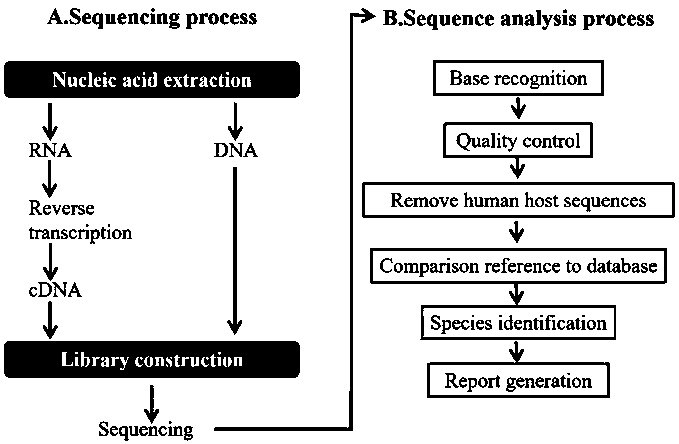
\includegraphics[width=0.6\textwidth]{img/analysis2}
    \caption{Phases comunes realizadas en un análisis de secuencias de ADN (Next-generation).}
    \label{fig:analysis}
\end{figure}


\section{Resultados}


\section{Conclusiones}

En este proyecto se ha desarrollado una herramienta distribuída que permite hacer el análisis masivo de grandes cantidades de lecturas de ADN (Next-generation sequencing). El objetivo fue demostrar que este análisis puede ser desarrollado utilizando Spark. \\

El proyecto se enfoco en el análisis de calidad de las lecturas de ADN, este es un paso crucial en cualquier experimento de Bioinformática. Como resultado, la propuesta obtiene estadísticas referentes a las ocurrencias de las bases nitrogenadas y además se desarrollo un análisis de contenido por base. \\
	
El proyecto esta es sus primeras etapas y en trabajos futuros se completará mas funcionalidades. El objetivo a largo plazo es desarrollar una herramienta distribuída que tenga las mismas actividades de las herramientas tradicionales.

\bibliographystyle{apalike}
%\bibliographystyle{IEEEtranN}
\bibliography{bibliography}

	
	
	
	
\end{document}